\documentclass{article}

\usepackage[spanish]{babel}
\usepackage{titling}
\usepackage{graphicx}
\usepackage{graphicx}
\usepackage[export]{adjustbox}
\usepackage{hyperref}
\usepackage{ragged2e}
\usepackage{indentfirst}
\usepackage{float}
\usepackage{microtype}
\usepackage[bottom]{footmisc}
\usepackage{fancyhdr}
\fancyhead[R]{2020}\fancyhead[L]{UNC - FCEFyN} \fancyfoot[C]{\thepage}
\pagestyle{fancy}

%%%%%%%%%%%%%%%%%%%%%%%%%%%%%%%%%%%%%%%%%%%%%%%%%%%%%%%%%%%%%%%%%%%%%%%%%%%%%%%

\title{Universidad Nacional de Córdoba\\Facultad de Ciencias Exactas, Físicas y Naturales}
\author{Tomas Sarquis}
\date{Diciembre 2020}

%%%%%%%%%%%%%%%%%%%%%%%%%%%%%%%%%%%%%%%%%%%%%%%%%%%%%%%%%%%%%%%%%%%%%%%%%%%%%%%

\hypersetup{
    colorlinks,
    citecolor=black,
    filecolor=black,
    linkcolor=blue,
    urlcolor=black
}

%%%%%%%%%%%%%%%%%%%%%%%%%%%%%%%%%%%%%%%%%%%%%%%%%%%%%%%%%%%%%%%%%%%%%%%%%%%%%%%

\newcommand{ \fnstackof }{\footnote{\url{www.stackoverflow.com/questions/63780850/esp32-best-way-to-store-data-frequently}}}
\newcommand{ \fnnvs }{\footnote{\url{docs.espressif.com/projects/esp-idf/en/latest/esp32/api-reference/storage/nvs_flash.html}}}
\newcommand{ \fnwifi }{\footnote{El sistema debía usar \emph{LoRa} pero el estudiante no contó con el \emph{hardware} necesario}}
\newcommand{ \fnsleep }{\footnote{El estudio del consumo considera únicamente las etapas de \emph{sleep} ya que en ésta etapa transcurre más del 90\% del programa}}
\newcommand{ \fnejemplos }{\footnote{\url{www.github.com/espressif/esp-idf/tree/master/examples/system/deep_sleep}}}
\newcommand{ \fnrepo }{\footnote{\url{www.github.com/tsarquis88/esp32_freertos}}}

%%%%%%%%%%%%%%%%%%%%%%%%%%%%%%%%%%%%%%%%%%%%%%%%%%%%%%%%%%%%%%%%%%%%%%%%%%%%%%%

\begin{document}

%%%%%%%%%%%%%%%%%%%%%%%%%%%%%%%%%%%%%%%%%%%%%%%%%%%%%%%%%%%%%%%%%%%%%%%%%%%%%%%

    \begin{titlingpage}
        \maketitle
        \null \null \null \null 
        
        \begin{center}
            {\huge Práctica Supervisada}
        \end{center}
        
        \begin{center}
            {\huge Segundas cien horas}
        \end{center}
        
        \topskip0pt % (?)
        
        \null \null \null \null 
        
        \begin{center}
            {\large \textbf{Monitoreo del movimiento de animales vacunos}}
        \end{center}
        
        \begin{center}
            {\large \textbf{Supervisor}: Gustavo Wolfmann }
        \end{center}

    \end{titlingpage}

%%%%%%%%%%%%%%%%%%%%%%%%%%%%%%%%%%%%%%%%%%%%%%%%%%%%%%%%%%%%%%%%%%%%%%%%%%%%%%%

    \tableofcontents 

%%%%%%%%%%%%%%%%%%%%%%%%%%%%%%%%%%%%%%%%%%%%%%%%%%%%%%%%%%%%%%%%%%%%%%%%%%%%%%%

    \newpage
    \section{Introducción}

    El presente documento detalla la realización de la práctica profesional
    supervisada llevada a cabo por el estudiante Tomas Sarquis, perteneciente 
    a la carrera de Ingeniería en Computación. \par

    La práctica profesional tuvo una duración de 200 (doscientas) horas, 
    repartidas en 41 (cuarenta y  uno) días. Este documento detalla la segunda
    mitad de la misma. \par

    En la documentación de la primera mitad de la práctica se ha comentando 
    acerca del objetivo de la misma y del entorno de trabajo, por lo tanto, 
    estos tópicos serán obviados en el presente documento.

%%%%%%%%%%%%%%%%%%%%%%%%%%%%%%%%%%%%%%%%%%%%%%%%%%%%%%%%%%%%%%%%%%%%%%%%%%%%%%%

    \newpage
    \section{Descripción del trabajo}   

    \subsection{Investigación}
    Si bien la etapa anterior de investigación abarcaba todas las necesidades,
    se tuvo que replantear ciertas cosas, por lo que la en la segunda parte se
    hizo inminente. \par
    Una de estas cosas fue el guardado en memoria de las mediciones. Después 
    de muchas idas y vueltas (en cuanto a qué tipo de memoria usar) se buscó
    respuestas en la comunidad, quién respondió satisfactoriamente. \fnstackof

    \subsection{Desarrollo}
    Habiendo terminado de configurar el sensor y de haber podido recibir de 
    manera exitosa las primeras mediciones de aceleración, lo siguiente era
    el guardado de las mismas y el posterior envío. 

    \subsubsection{Almacenamiento}
    El microcontrolador cuenta con distintas maneras de almacenar datos. \par
    Primeramente se optó por utilizar la memoria \emph{NVS}\fnnvs 
    (``Almacenamiento no volátil``) por su facilidad, pero se tuvo que pensar 
    en otra manera debido a que este método utliza la memoria \emph{Flash}, y 
    el uso constante de la misma tiende a degradarla. \par
    Finalmente, con ayuda del supervisor de práctica, se decidió por usar un 
    sistema (figura \ref{fig:memoria}) de memorias de dos niveles: los datos 
    recibidos desde el sensor se van acumulando en la memoria \emph{RTC RAM} 
    del microcontrolador (que no se degrada con el uso), y cuando ésta se 
    llena, se transfieren los datos al \emph{filesystem SPIFFS} (que tiene 
    muchas más capacidad de almacenamiento), dejando vacía la primera. 
    Luego se vuelve a usar la \emph{RTC RAM}, y el proceso se repite hasta 
    que el \emph{filesystem} agota su capacidad. \par
    El sistema \emph{SPIFFS} utliza la memoria \emph{Flash}, pero como está
    en un ``segundo nivel``, no se escribe tan seguido y por lo tanto, no 
    se degrada tan rápidamente. \par
    Cuando el \emph{filesystem} se llena, se debe vaciar y transferir los
    datos al servidor. \par
    Se busca que el envío de las mediciones no se realice de manera frecuente, 
    ya que el consumo de energía se vería afectado negativamente. Es por esto
    que se intentó aprovechar al máximo la fase de almacenamiento.

    \begin{figure}[h]
        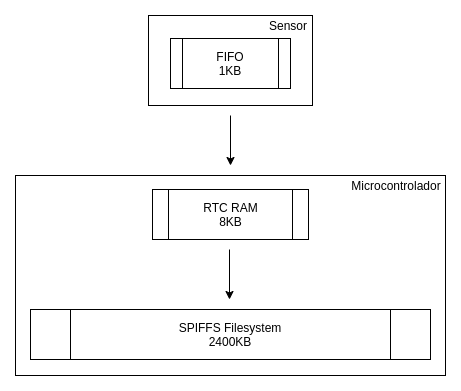
\includegraphics[width=0.8 \textwidth, center]{esquema_memoria.png}
        \caption{Esquema de memoria en niveles}
        \label{fig:memoria}
    \end{figure}

    \subsubsection{Transferencia}
    La idea es que, cuando sea necesario, se pueda enviar todas las mediciones
    a un servidor de la red local (en un \emph{drone} que circula cerca) de 
    forma segura. Para esto, se usó el protocolo \emph{HTTP}, mientras que 
    la tecnología inalámbrica fue \emph{Wi-Fi}\fnwifi. \par
    La transferencia consiste en varios paquetes \emph{HTTP} de tamaño 
    configurable. Para las pruebas se han usado paquetes de 100 datos cada uno.

    \begin{figure}[h]
        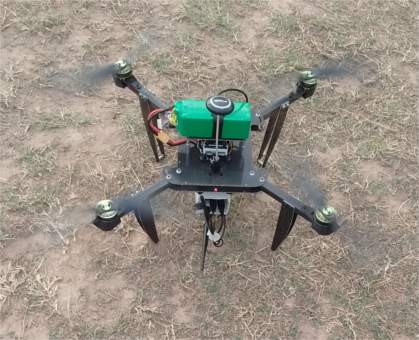
\includegraphics[width=0.8 \textwidth, center]{drone.jpg}
        \caption{\emph{Drone} funcionando como servidor}
        \label{fig:drone}
    \end{figure}

    \subsubsection{FreeRTOS}
    El sistema operativo que orquesta el sistema es \emph{FreeRTOS}, el cuál
    estuvo diseñado por 3 tareas:
    \begin{itemize}
        \item \textbf{Tarea principal:} Encargada de crear las demás tareas y 
        los recursos compartidos.
        \item \textbf{Tarea de acelerómetro:} Su misión es la de recepción y 
        almacenamiento de las mediciones.
        \item \textbf{Tarea de transferencia:} Realiza las tareas de envío
        de datos al servidor.
    \end{itemize}

    \subsection{Resultados}
    Los resultados a continuación detallados han sido recavados de la ejecución
    del sistema en el \emph{Intelytrace} y no en la placa de pruebas.

    \subsubsection{Mediciones}
    Los resultados arrojados se pueden observar en la figura 
    \ref{fig:resultados_modulo}, los cuales fueron obtenidos midiendo la 
    aceleración humana caminando y trotando a distintas velocidades. La 
    cantidad de mediciones es de 1488.

    \begin{figure}[h]
        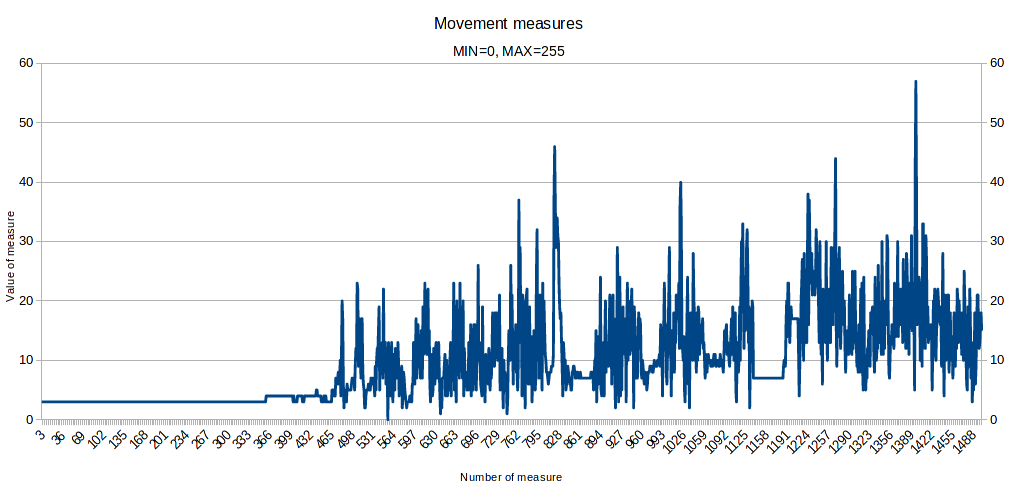
\includegraphics[width=1.0 \textwidth, center]{results_module.png}
        \caption{Resultados obtenidos}
        \label{fig:resultados_modulo}
    \end{figure}

    \subsubsection{Consumo}
    Uno de los requisitos principales era que el consumo de la placa sea lo 
    menor posible y para esto se hizo incapié en que el microcontrolador se 
    encuentre en modo \emph{sleep} la mayor parte del tiempo.\fnsleep \par
    A pesar de esto, los resultados obtenidos en cuanto al amperaje no fueron
    los esperados, como se puede ver en la tabla \ref{tab:consumo}. \par
    Cabe aclarar que la corriente eléctrica (consumo) fue medida en serie
    a la batería que alimenta toda la placa.

    \begin{table}[h]
        \centering
        \begin{tabular}{||c|c||} 
            \hline
            Consumo esperado & Consumo obtenido \\ [0.5ex] 
            \hline\hline
            10 [uA] & 4.3 [mA] \\
            \hline
        \end{tabular}
        \caption{Consumo esperado y obtenido (\emph{deep-sleep mode})}
        \label{tab:consumo}
    \end{table}

    Si bien no se sabe, a ciencia cierta, a qué se debe esta diferencia de 
    consumo, la misma no se atribuye a un problema del \emph{software} 
    implementado, ya que se han llevado a cabo pruebas con programas 
    oficiales\fnejemplos y los resultados han sido los mismos. \par
    Por su parte, la placa incrustada en el \emph{Intelytrace} no solo cuenta 
    con el ESP32, si no que cuenta, además, con otros componentes de 
    \emph{hardware} como cargador de batería, receptor LoRa WAN y GPS, por lo 
    que se plantea como hipótesis que dichos componentes sean los causantes del 
    alto consumo, y no el ESP32 propiamente dicho.

%%%%%%%%%%%%%%%%%%%%%%%%%%%%%%%%%%%%%%%%%%%%%%%%%%%%%%%%%%%%%%%%%%%%%%%%%%%%%%%

    \newpage
    \section{Conclusión}

    La práctica supervisada ha sido una actividad realmente enriquecedora tanto
    para el alumno como para el supervisor y su empresa. El estudiante tuvo una
    experiencia real de la implementación completa de un \emph{software}, 
    pasando por el análisis de los requerimientos, el diseño, las posibilidades
    de desarrollo, las investigaciones posteriores y finalmente el desarrollo y
    los resultados. \par
    El sistema implementado en estos meses es susceptible a (y debería, en lo 
    posible) ser mejorado, ya que ciertas cuestiones del programa lo ameritan.
    Además, se recomienda hacer más pruebas de \emph{testing}, ya que el 
    desarrollador pudo hacer solamente las pruebas básicas. \par
    Algunas mejoras podrían ser:
    \begin{itemize}
        \item Reemplazar la conexión WiFi por LoRa WAN
        \item Tener en cuenta valores de movimiento relativos. Esto es, no solo
        tener en cuenta los valores absolutos, si no, además, computar las 
        diferencias de movimiento en función del tiempo. Esto podría ser útil
        para detectar cambios bruscos de movimiento.
        \item Arreglo de \emph{bugs}
    \end{itemize} \par
    A pesar de esto y teniendo en cuenta el tiempo empleado para el desarrollo 
    y la poca experiencia del desarrollador, el resultado es muy favorable: los
    requerimientos fundamentales han sido satisfechos. \par
    Los conocimientos obtenidos en la universidad y las ayudas recibidas por
    parte del supervisor y de la comunidad informática, fueron de necesidad para
    el estudiante.

%%%%%%%%%%%%%%%%%%%%%%%%%%%%%%%%%%%%%%%%%%%%%%%%%%%%%%%%%%%%%%%%%%%%%%%%%%%%%%%

\newpage
\section{Apéndice}

El código del programa implementado se puede apreciar en el repositorio\fnrepo 
del desarrollador. Los archivos de interés se encuentran
sobre el directorio \emph{esp-idf/main} que, a su vez, contiene tres 
directorios más:
\begin{itemize}
    \item \emph{include}. Contiene los \emph{headers} del código fuente.
    \item \emph{lib}. Dentro se encuentran las librerías externas que han sido 
    usadas.
    \item \emph{src}. El código fuente de cada tarea se encuentra aquí.
\end{itemize} \par
El área de mayor interés es, quizás, la del directorio \emph{src}. En él se 
encuentran implementadas las tareas del sistema, por lo que para conocer su
funcionamiento, es de crucial importancia entender estos códigos.

%%%%%%%%%%%%%%%%%%%%%%%%%%%%%%%%%%%%%%%%%%%%%%%%%%%%%%%%%%%%%%%%%%%%%%%%%%%%%%%

\end{document}